\section{Results}
\label{sec:results}

\todo{This is the results section}

We present a comparison between the usage characteristics of the control\footnote{gateway byte counters from users with a 105 Mbps access link} and test\footnote{gateway byte counters from users with a 105 Mbps access link}. We interpret the results as change in usage behavior due to increase in access link bandwidth. %although these are two separate sets of devices we interpret them as changes as explained in "methodology" or "data"

\subsection{User Behavior}
\label{subsec:behavior}

\hypoth{1}. Does aggregate user behavior differ?

\begin{figure}[t!]
%\hspace*{-0.2in}
\begin{minipage}{1\linewidth}
\centering
%
%\hfill
\begin{subfigure}[b]{0.5\linewidth}
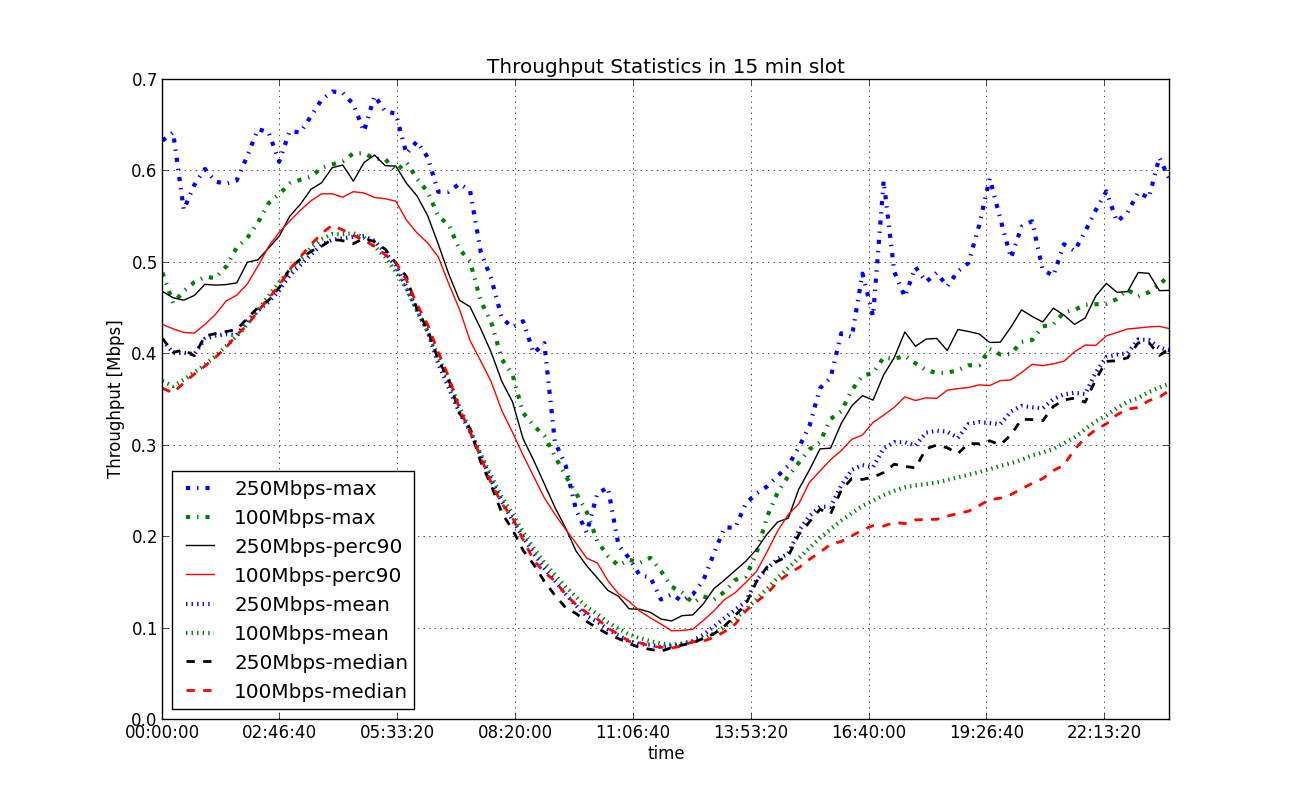
\includegraphics[width=\linewidth]{figures/describe-total-throughput-per-day[replace].png}
  \caption{Old plot of daily agg (over days) of means (over devices)}
  %http://riverside.noise.gatech.edu:8083/separated/full/describe-total-throughput-per-day.png
  \label{fig:TS-data-rate-daily}
\end{subfigure}
%
\hspace{-1em}
%
\begin{subfigure}[b]{0.5\linewidth}
\includegraphics[width=\linewidth]{figures/.png}
  \caption{CDF of data rate per time slot for all devices (agg view of data)}
  %http://sites.noise.gatech.edu/~sarthak/files/comcast/plots/full_dw/cdf-all-bytes.png
  \label{fig:CDF-data-rate-all}
\end{subfigure}
%\hfill
%
\end{minipage}
\caption{User Behavior: Overall not much change due to capacity increase}
\label{fig:user-behavior}
% created using docs/metadata-separated.log
\end{figure}


\subsection{Peak Utilization}
\label{subsec:peak-util}

\hypoth{2}. Does the maximum (or 90-\%ile) data transferred by the device differ?

\subsection{Prime Time Ratio}
\label{subsec:prime-time}

\hypoth{3}. Does the prime-time ratio differ?

\subsection{Peak Ratio}
\label{subsec:peak-ratio}

\hypoth{4}. How much does the traffic vary in a single day?


\subsection{Traffic Asymmetry}
\label{subsec:asymmetry}
\todo{maybe this doesn't need a separate section, just comment on asymmetry in each of the above - plot uplink also}
